\documentclass{article}
\usepackage{lmodern}
\usepackage[T1]{fontenc}
\usepackage{amsfonts} % \mathbb
\usepackage[margin=0.5in]{geometry}
\usepackage[utf8]{inputenc}
\usepackage{graphicx}
\usepackage[backend=biber, style=apa]{biblatex}
\usepackage{amsmath}
\DeclareMathOperator{\sign}{sign}
\bibliography{bibli}

\title{Robust Digital Envelope Estimation Via Geometric Properties of an Arbitrary Real Signal}
\author{
  Carlos Tarjano
  \and 
  Valdecy Pereira
  }

\begin{document}

\maketitle

\begin{abstract} % 250 words

% estimate parameters from the signal itself
% broadband
% Dominant frequency as by-product
% we define several entities in the process, introducing a new measure of discrete curve curvature, hoping to consolidate the terminology in the area

  % background  
  Despite being an elusive concept, mathematically well defined only for artificially generated waves, the temporal amplitude envelope of a signal is essential for its complete characterization, being the primary information carrying medium in spoken voice and telecommunications, for example.
  intuitively, the temporal envelope can be understood as a smooth function on the same variable as the principal wave, or temporal fine structure, that modulates the signal, responsible for its outer shape. It is implied in this definition that the envelope is non periodic in general and is thus better addressed by specific techniques diverse from those used in the analysis of the periodic, rapidly changing wave it encompasses.
  % motivation
  Envelope detection techniques have applications in areas like health, sound classification and synthesis, seismology and speech recognition. Despite of that, a general approach to envelope detection of signals with rich spectral content seems to be lacking, and most methods involve manual intervention, like filter design, based on prior knowledge about the wave under investigation.
  % objective
  In this paper we propose a framework that uses intrinsic characteristics of a signal to estimate its envelope, eliminating the necessity of parameter tuning.
  % methods
  The approach here described draws inspiration from general, computational and differential geometry to isolate the frontier of an arbitrary signal. The concepts of alpha-shapes, concave hulls, arc-length parametrization and discrete curve curvature are adapted. We also define a pulse in the context of a arbitrary digital signal as a means to reduce dimensionality and the complexity of the proposed algorithm.
  % results
  
  % implications

\end{abstract}

{\bf Keywords:} DSP, alpha-shapes, envelope detection

\section{Introduction} % 500 words
% Opener sentence
Despite being ubiquitous in digital signal processing, the literature about envelope detection is very fragmented \parencite{2017LyonsDigital}. Besides, most envelope detection techniques are designed to account for very specific settings, like pure sinusoids with moderate noise contents, in line with the most common usages of those algorithms with artificial signals in the context of analog telecommunications.

% Literature review | Brief Context of Prior Research
In many natural signals, however, the temporal amplitude envelope of a signal plays a prominent role in the characteristics exhibited: According to \textcite{2017QiRelative}, for example, the envelope is at least as important as the fine structure of the soundwave in the context of the intelligibility of mandarin tones. That is also the case for English \parencite{1995ShannonSpeech}, where even envelopes modulating mostly noise were still capable of conveying meaning. The envelope helps to convey emotion and identity to the human voice \parencite{2018ZhuContributions}, and envelope preserving characteristics of concert halls are associated with their pleasantness \parencite{2011LokkiEngaging}.

% Cite current algorithms
When dealing with broadband signals, approaches tailored to specific applications are prevalent, such as the one presented by \textcite{2014YangFast} for the distributed monitoring of fibre optic or the one formulated by \textcite{2018AssefModeling} in the context of medical ultrasound imaging.

If one adresses the different units in the horizontal and vertical axes, one can transform the DSP problem of envelope detection in the geometric problem of defining the shape of a set of points in $ \mathbb{R}^2 $. For that purpose \textcite{1983Edelsbrunnershape} introduced the concept of alpha-shapes, a mathematically well defined extension to the convex hull of a finite set of points, related to the Delaunay triangulation and Voronoi diagrams of those points.

This approach is used in areas such as the detection of features in images \parencite{2016VarytimidisAlpha}, reconstruction of surfaces from a cloud of points \parencite{2015WuAutomated} and Spectroscopy \parencite{2019XuModeling}, with the last work, that involves the estimation and removal of the Blaze function (a kind of envelope) of a echelle spectrograph, being particularly align with what is intended here.

% Restate Your Question as Something Not Known or Fully Understood by Prior Research
Thus, in this paper we formulate a general approach to envelope detection, exploiting the intrinsic characteristics of a generic, spectrally complex, wave in order to avoid the need to manual intervention or parameter tuning.

% State the Significance of Your Question
While the robustness of the proposed approach allows it to be used as a plug in replacement for many methods encountered in the literature, we feel that it would be particularly useful for sound synthesis. 
The envelope is shown to add complexity to the spectral representation of a wave \parencite{2019TarjanoNeuro}, and a accurate description of the envelope would be useful for a cleaner spectral analysis. Moreover, the algorithm naturally divides a signal in pseudo-cycles, that could serve pragmatic building blocks for the reconstruction of the fine structure of the wave.

% State Your Claim | Objective | Hypothesis
In the context of sound synthesis, one would be able to apply specific methods for the recreation of the envelope, more in line with its smooth, slow varying and non periodic nature and a different approach to the periodic and relatively fast changes of the temporal fine structure.
% TODO brief outlook on the structure of the paper


\section{Methodology} % 1000 words

% Essential background information
We start by defining a pulse as a series of consecutive samples in a discrete wave with the same sign. More formally, let $ W[i] \in \mathbb{R} \forall i \in \mathbb{N}_0, i < n \in \mathbb{N}_0 $ be a real, discrete and finite signal indexed, without loss of generality, over a subset of the natural numbers. This definition relates closely to the concept of an array or vector in most programming languages, and is used in the interest of simplicity. 

A pulse $ P[j], j \in \mathbb{N}_0, j < q $ in $ W $ can then be defined as a sequence of samples indexed by $ i $ such that $ \sign(W[a-1]) \ne \sign(W[a]) = \sign(W[a+1]) = \dots = \sign(W[b-1]) = \sign(W[b]) \ne \sign(W[b+1]) \forall i, a \le i \le b | a,b \in \mathbb{N}_0 $.

In other words, each pulse is a unique subset of $ W $ with its members being the maximum sequence of samples in $ W $ with the same signal and $ P[0] \cup P[0] \cup \cdots \cup P[q-1] = W $. It is convenient to attribute to each pulse a pair of coordinates: those will be the coordinates of the sample with the maximum amplitude in each pulse.

Naturally, each pulse can be classified as positive or negative, based on the signal of its samples, which must be the same.
For a continuous function, then, a pulse would correspond to the pieces between it's roots, and would be equal to half the cycle of a sinusoid. Thus, in our analogy, two consecutive pulses, naturally with opposing signs, have the potential do delimitate a pseudo-cycle, as illustrated in figure \ref{fig:Pulses}. For that to be true, however, the pulses need to make part of the frontiers of the signal, as will be defined later.

  \begin{figure}[ht!]
    \centering
      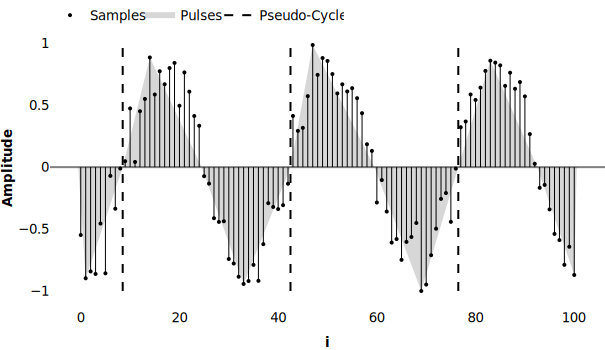
\includegraphics[width=0.8\linewidth]{01Pulses.pdf}
    \caption{The grey areas encompass the simplified convex hulls of the pulses. The dashed lines mark the frontier between pseudo-cycles.}
    \label{fig:Pulses}
  \end{figure}

The most mathematically sound definition of an envelope involves its representation as an analytic signal, introduced by Gabor in 1946 \parencite{2007HahnHistory}. In his work, \textcite{1946GaborTheory} applies the then relatively new mathematical machinery of the quantum mechanics to unify time and frequency representations of a wave, showing how the Hilbert transform could be applied to a real signal in order to obtain a complex signal that would become known as the analytic signal.

This analytic signal is of the form $ a(t) = s(t) + j \mathbb{H}(s(t)) $ \parencite{2016HePraat} where $ s(t) $ is the original real signal, that becomes the real part of the analytic signal. $ \mathbb{H}(s(t)) $, the Hilbert transform of the original signal becomes, then, the imaginary part of the analytic signal; the envelope of a signal thus represented can be straightforwardly obtained by the computation of its complex modulus.

\begin{figure}[ht!]
  \centering
    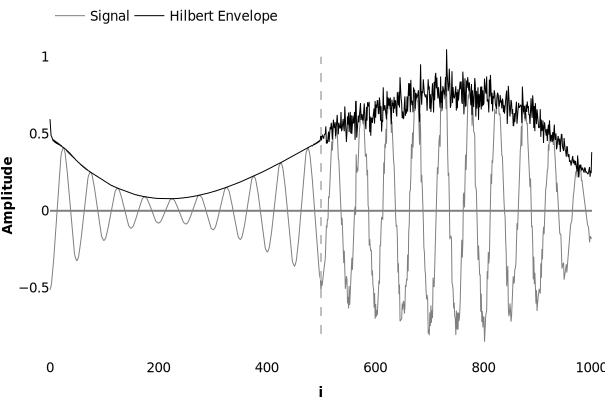
\includegraphics[width=0.8\linewidth]{02AnalyticSignal.pdf}
  \caption{Envelope of a pure sinusoid modulated by a polynomial of degree 3, as obtained by the Hilbert Transform. In the first half the sinusoid is free of noise, while in the second half white gaussian noise with a standard deviation of $ 1/10 $ of the maximum amplitude of the wave was added to the base signal.}
  \label{fig:AnalyticSignal}
\end{figure}

Figure \ref{fig:AnalyticSignal} shows the envelope obtained via the Hilbert transform, for a pure sinusoid of local frequency 20, modulated by a polynomial of the third degree, in the presence and absence of gaussian white noise with standard deviation of $ 1/10 $ of the wave's maximum amplitude. It is readily noticeable that, as soon as noise is introduced in the original signal, it is reflected in the envelope, breaking our assumption of smoothness. Other than that, this definition yields a unique, positive envelope.

In practice, however, is not uncommon for a discrete wave, specially in the case of sound, to present somewhat different positive and negative contours; as our method will forcibly have to be applied separately to both sides, superior and inferior, of the discrete wave, it is only natural to introduce such separation as soon as possible. 

To do so we will define the positive (upper) frontier and negative (lower) frontier as the set of points $ (i, |W[i]|) $ that are, necessarily but not sufficiently, the point of maximum amplitude of their respective pulses. The set of all these points such that $ W[i] > 0 $ will be called the positive, piecewise linear frontier and will be denoted by $ F_+ $; similarly, $ F_- $ will denote the negative frontier of $ W $, defined by the subset of points $ (i, W[i]) $ where $ W[i] < 0 $, as is shown in figure \ref{fig:Frontiers}. To identify such points, we need to address the different units in which the amplitude and horizontal distance of our wave are expressed.

\begin{figure}[ht!]
  \centering
    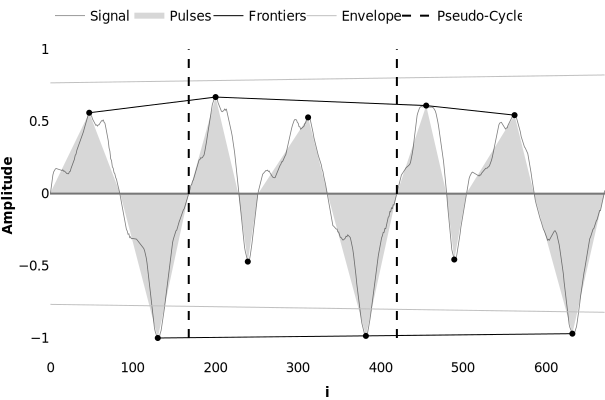
\includegraphics[width=0.8\linewidth]{03Frontiers.pdf}
  \caption{Positive and negative frontiers, envelope and pseudo-cycles for a fragment of piano sound. While we have only one (positive) envelope, here mirrored in the inferior space, we have two frontiers, the superior and inferior.}
  \label{fig:Frontiers}
\end{figure}

To make abscissa and ordinate units consistent for the computation of the frontier, and proceed with a geometric treatment of the subject, we consider the set of positive and negative pulses separately. For each set, we multiply all pulses by the average length of the pulses in the set, after having divided by the average of the pulses' amplitudes, putting both axes in the same frame related unit $i$, related to time by the equation $i = t \ \mathit{fps}$.

Because we are interested in approximating a function that is smooth over the whole domain of the wave, we can assume that, in the scale of a pulse, this function will be very close to a horizontal straight line and, thus, won't touch any point inside the convex hull defined by the pulse. 

By the same token, as the change in amplitude from one pulse to the next pulse with the same sign is motivated by changes in this same envelope, one can reasonably suppose that $ \max(P[j]) \approx \max(P[j+2]) $. That justifies the approximation of the convex hull of a pulse by the triangle defined by the points where the pulse crosses the horizontal the point of maximum amplitude; this will allow a considerable dimension reduction as this triangular pulse can become the atomic unit for the rest of the method. 

This definition also makes clear that only one point of an arbitrary pulse can be in the frontier, namely, its point of maximum amplitude; those definitions will allow us to derive the frontiers of a wave using an alpha-shapes inspired algorithm without the need to compute the Delaunay triangulation first.

Translating the intuitive explanation of alpha-shapes in \textcite{1994EdelsbrunnerThree} to our context, we can say that the points in the frontier are those touched by a circle outside the signal that is not allowed to contain any point of the signal; The pulses that contain said points can be seen as frontier pulses.
Intuitively, one can picture a circle being rolled above (or below, in the case of the negative frontier) the signal, and marking the points it touches as frontier points.

We can therefore revisit the concept of a pseudo-cycle, only hinted at before, defining it as the samples of the original wave that belong to two successive pulses that belong to their respective frontiers, including eventual pulses between them, as can be seen in figure \ref{fig:Frontiers}.

% TODO snowball image

It is now necessary to infer the appropriate radius of such a circle and, to that end, a measure of the curvature of a discrete function is needed. Discrete curvature estimation is an important task in image processing \parencite{2010FleischmannNovel} for which no default definition exists; The two possible approaches are the derivation of direct methods that use characteristics of the discrete wave to calculate its curvature at each point, or the calculation of the curvature of a curve fitted to the discrete wave \parencite{2001CoeurjollyDiscrete}.

To fit a polynomial to the a generic wave two approaches are readily available: the least mean squares approach, that seeks to minimize the dependant variable errors and the total least squares problem, that treats both variables symmetrically \parencite{1980GolubAnalysis}.

The geometric, symmetrical nature of the problem excludes the more computationally economic least mean squares approach however, leaving us with the total least squares, for which no general closed form solutions are available \parencite{2007MarkovskyOverview}; this leads us to turn our attention to direct approaches of curvature estimation.

\subsection{Discrete Curvature Estimation - The Equivalent Circle Approach}

As previously stated, no default discrete curvature definition exists; \textcite{2014CarrollSurvey}, for example, derives 3 such different definitions based on the approximation of a circle by an inscribed, centred e circumscribed polygon. In the context of 3d meshes, \textcite{2016VasaMultivariate} evaluate a range of estimators from a multivariate point o view.

For our needs, however, it is more convenient to define our own discrete curvature estimator; the approach here presented differs from most others found in the literature in that the curvature is defined over the edges linking the points that form the discrete wave, instead of the vertices.

To that end we are going to apply the definition of smooth curvature as the rate of change of the unit tangent to a curve, noting that this is equivalent to that of the osculating circle \parencite{2016VasaMesh}.
The idea is to find the equivalent circle whose tangent presents the same change in direction, in the same horizontal distance, as the edge of interest. This approach presents the convenience of estimating the radius directly.

\begin{figure}[ht!]
  \centering
    \includegraphics[width=0.5\linewidth]{04DiscreteCurvature.pdf}
  \caption{Change of direction from horizontal, in $x_0$, until an angle of $\theta$, in $x_1$, that is equivalent to the angle between the average direction and the direction of the vector $\vec{v}[l]$ whose radius of curvature is being calculated. $x_0$ and $x_1$} correspond to the the horizontal coordinates of the tale and tip of $\vec{v}[l]$, respectively.
  \label{fig:DiscreteCurvature}
\end{figure}

Formally, for each frontier, positive or negative, we define $ m - 1 $ vectors, $ m $ being the number of positive or negative pulses respectively, as the coordinates of the posterior pulse with the relevant signal minus the preceding pulse: $\vec{v}[l]^\pm = (P[l+1]_x^\pm - P[l]_x^\pm, P[l+1]_y^\pm - P[l]_y^\pm), \forall 0 \le l < m - 1 $, recalling that the $x$ coordinate of a pulse was defined as the $x$ coordinate of its sample with maximum amplitude, while the $y$ coordinate of a pulse is this amplitude itself.

Since an edge defines only one direction, there remains the need for a reference. As we are interested in the relative curvature, it is natural to use the average direction of all vectors, $ \vec{\overline{v}}^\pm = \frac{1}{m-1} \sum_{l=0}^{m-1} \vec{v}[l]^\pm $, so as to measure the relative change of direction of each edge. This procedure, as well as the circles generated by it, are illustrated in figure \ref{fig:Curvatures}

\begin{figure}[ht!]
  \centering
    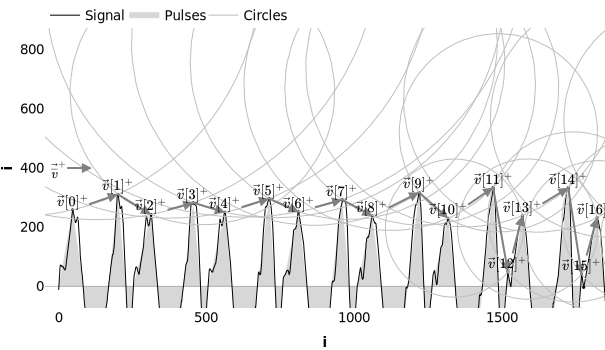
\includegraphics[width=0.8\linewidth]{05Curvatures.pdf}
  \caption{The equivalent circles obtained via the procedure described for the positive frontier. $\theta$, the angle between $ \vec{\overline{v}}^+$ and each of the $\vec{v}[l]^+$ is used, as is the horizontal component of each $\vec{v}[l]^+$ to obtain the radii of the circles.}
  \label{fig:Curvatures}
\end{figure}

After this procedure one obtains a set of points in $ \mathbb{R}^2 $ % TODO

\begin{figure}[ht!]
  \centering
    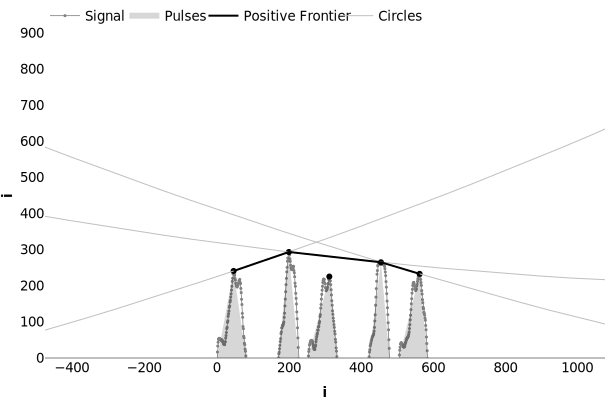
\includegraphics[width=0.8\linewidth]{06AvgCircle.pdf}
  \caption{The positive frontier as obtained by the use of the circle representing the average curvature of the discrete wave illustrated.}
  \label{fig:AvgCircle}
\end{figure}

% Therefore, the definition of the curvature becomes $ \kappa(x) = \frac{2 a}{\big( (b + 2 a x)^2 + 1 \big)^\frac{3}{2}} $ with the average curvature between points $ x_0 $ and $ x_1 $ given by equation \ref{eq:1}.

% \begin{equation} \label{eq:1}
%   \overline{\kappa}(x) = 
%   \frac{
%       \left( \dfrac{2 a x_1 + b}{\sqrt{\big(2 a x_1 + b \big)^2+1}} - \dfrac{2 a x_0 + b}{\sqrt{\big(2 a x_0 + b \big)^2+1}} \right) 
%   }{
%     (x_1 - x_0)
%   }
% \end{equation}

% \subsection{Theory}


  
\section{Results}

\subsection{Robustness}

\subsection{Fundamental Frequency as a Welcome Side-effect}

\section{Discussion + Conclusion}

\section{References}
\printbibliography[heading=none]

\end{document}
